
\documentclass{article}

\usepackage{graphviz}
\usepackage{url}
\usepackage{hyperref}
\usepackage{fullpage}
\usepackage{parskip}
\usepackage{fancyvrb}
\usepackage{amsmath}
\usepackage{framed}

\usepackage{listings}
\lstset{numbers=left,
		basicstyle=\footnotesize,
		captionpos=b,
		xleftmargin=0.3in}

%
% backend	: biber
% style		: numeric
% autocite	: footnote
% citestyle	: verbose-inote
% bibstyle	: authortitle, numeric
%
\usepackage[backend=biber,autocite=footnote,
			bibstyle=authortitle,citestyle=verbose-inote]{biblatex}

\addbibresource{references.bib}
\setlength\bibitemsep{1em}

\providecommand{\e}[1]{\ensuremath{\times 10^{#1}}}

\VerbatimFootnotes

\raggedright

% Change enumerate section numbering
\renewcommand*{\theenumii}{\theenumi.\arabic{enumii}}
\renewcommand*{\labelenumii}{\theenumi.\arabic{enumii}}

\begin{document}

% {{{ title page
\vspace*{1.0in}

\centerline{\LARGE \textbf{SprinklerPI}}
\vspace{0.3in}
\centerline{\LARGE Product Test Plan}

\vfill

\begin{center}
\begin{tabular}{c}
\today \\
\href{http://github.com/jmmahler/sprinklerpi}{github.com/jmmahler/sprinklerpi}
\end{tabular}
\end{center}

\vspace{2in}

\thispagestyle{empty}

\pagebreak
% }}}

\thispagestyle{empty}
\tableofcontents
\clearpage

% {{{ Information Required for Execution
\section{Information Required for Execution}

\subsection{Purpose}

The purpose of this test protocol is to verify the full and complete
operation of the SprinklerPI system.

\subsection{Scope}

This test protocol should be executed to verify that each principal feature
and function performs within specification called out by the engineering
requirements document. In addition, other necessary specifications shall
be tested such as specific and necessary user, installation and power
requirements. The testing called out in this protocol is subject exclusively
to those selected specifications provided for the SprinklerPI.

\subsection{Responsibilities}

It is the responsibility of the assigned test engineer to execute all tests
included herein to the best of their ability. If necessary, seek additional
assistance to execute tasks.

%\subsection{Definitions}

\subsection{Equipment/Supplies}

\begin{itemize}
\item 110 volts AC power supply (NEMA 5-15R).
\item Digital volt meter.
\item Three test bridges (25 $\Omega$, 50 watt).
\item PC with internet access and a web browser.
\end{itemize}

\subsection{Precautions \& Warnings}

This test plan contains certain warnings and cautions that the test
engineer must be aware of while performing these tests.
The following illustrates each of these messages and how to recognize them.

\fbox{
\textbf{WARNING: \textless message\textgreater}
}

The ``WARNING: Message'' alerts the user about safety issues that are of
the highest importance, such as possible injury to the operator.

\fbox{
\textbf{CAUTION: \textless message\textgreater}
}

The ``CAUTION: Message'' alerts the user to issues concerning possible
damage to the equipment or that can lead to erroneous test results.

% }}}

\pagebreak

% {{{ Testing Features and Functions
\section{Testing Features and Functions}

This test procedure is used to determine if the system,
as shown in Figure \ref{fig:all}, is fully functional and operating
within allowable tolerances.

\begin{figure}[h!]
\begin{center}
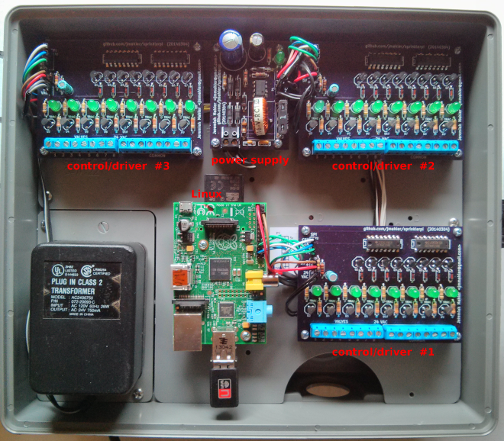
\includegraphics[scale=0.7]{img/all-inst-03.png}
\end{center}
\caption{Overview of the major components of the SprinklerPI system.
Green LEDs are used to indicate operation.
The power supply has an LED in the top right.
And each of the control/driver outputs has an corresponding LED.}
\label{fig:all}
\end{figure}

It is assumed that the SprinklerPI software has been installed
and networking has been configured according to the \verb+README+
included with the project\autocite{sprinklerpi}.

\pagebreak

% {{{ Power On Test
\subsection{Power On Test}

\begin{enumerate}
\item Equipment Required
	\begin{itemize}
		\item 110 volts AC power outlet (NEMA 5-15R).
	\end{itemize}
\item Input
	\begin{itemize}
	\item 110 volts AC
	\end{itemize}
\item Output
	\begin{itemize}
	\item Green power LED on.
	\item Activity LEDs during boot up.
	\item Control LEDs off.
	\end{itemize}
\item Test Description \\
\vspace{0.5em}

After plugging in the cord to a 110 volt AC outlet the green LED on
the power supply should go on (Figure \ref{fig:all}).
Then, as the Linux computer boots up, activity should be seen on its LEDs.
The LEDs on the control/driver boards may go on/off randomly as the
system boots.  Valve number one may be on during most of the boot,
this is normal.
After approximately 30 seconds the activity on the LEDs on the Linux
computer should be stabilize, indicating that the system has completed booting.
At this point all the control/driver LEDs should be off.

\item Test Results \\
\vspace{1em}
\begin{tabular}{|l|l|l|l|}
	\hline
	\multicolumn{1}{|c|}{Test}
	& \multicolumn{1}{|c|}{Value}
	& \multicolumn{1}{|c|}{Pass/Fail}
	& \multicolumn{1}{|c|}{Notes} \\
	\hline
	Power LED on? & on & P \quad F & \hspace{1.7in} \\
	\hline
	Activity LEDs during boot? & yes & P \quad F & \\
	\hline
	Stable activity LEDs after boot up? & yes & P \quad F & \\
	\hline
	Control outputs off after boot up? & yes & P \quad F & \\
	\hline
\end{tabular}

\end{enumerate}
% }}}

% {{{ Manual Control Test
\clearpage
\subsection{Manual Control Test}
\label{sec:manual-control-test}

\begin{enumerate}
\item Equipment Required
	\begin{itemize}
	\item 110 volts AC power outlet (NEMA 5-15R).
	\item PC with Internet access and a web browser.
	\end{itemize}
\item Input
	\begin{itemize}
	\item User turns valves on using manual mode of web interface.
	\end{itemize}
\item Output
	\begin{itemize}
	\item LED indicator for each valve which is turned on.
	\end{itemize}
\item Test Description \\

This test verifies that the valves can be manually operated from
the web interface (Figure \ref{fig:www-manual_mode}).
The user iterates through each possible combination and verifies
that the LED indicator for the corresponding valve is on.

\begin{figure}[hbp!]
\begin{center}
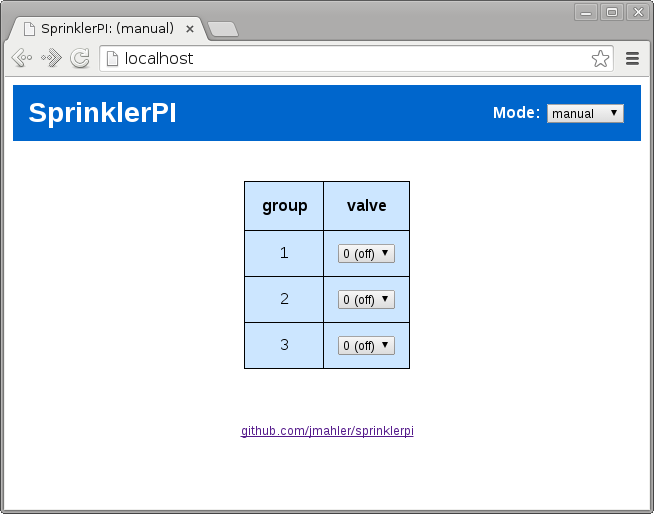
\includegraphics[scale=0.5]{img/www-manual_mode}
\end{center}
\caption{Web interface in manual mode which allows operation of
a single valve for each group.}
\label{fig:www-manual_mode}
\end{figure}

\pagebreak
\item Test Results \\
	\vspace{1em}
	\begin{tabular}{|c|c|c|c|c|}
		\hline
		Group & Valve & Value & Pass/Fail & Notes \\
		\hline
		1 & 0 & off & P \quad F & \hspace{20em} \\
		\hline
		1 & 1 & on & P \quad F & \\
		\hline
		1 & 2 & on & P \quad F & \\
		\hline
		1 & 3 & on & P \quad F & \\
		\hline
		1 & 4 & on & P \quad F & \\
		\hline
		1 & 5 & on & P \quad F & \\
		\hline
		1 & 6 & on & P \quad F & \\
		\hline
		1 & 7 & on & P \quad F & \\
		\hline
		1 & 8 & on & P \quad F & \\
		\hline
		\hline
		2 & 0 & off & P \quad F & \\
		\hline
		2 & 1 & on & P \quad F & \\
		\hline
		2 & 2 & on & P \quad F & \\
		\hline
		2 & 3 & on & P \quad F & \\
		\hline
		2 & 4 & on & P \quad F & \\
		\hline
		2 & 5 & on & P \quad F & \\
		\hline
		2 & 6 & on & P \quad F & \\
		\hline
		2 & 7 & on & P \quad F & \\
		\hline
		2 & 8 & on & P \quad F & \\
		\hline
		\hline
		3 & 0 & off & P \quad F & \\
		\hline
		3 & 1 & on & P \quad F & \\
		\hline
		3 & 2 & on & P \quad F & \\
		\hline
		3 & 3 & on & P \quad F & \\
		\hline
		3 & 4 & on & P \quad F & \\
		\hline
		3 & 5 & on & P \quad F & \\
		\hline
		3 & 6 & on & P \quad F & \\
		\hline
		3 & 7 & on & P \quad F & \\
		\hline
		3 & 8 & on & P \quad F & \\
		\hline
	\end{tabular}
\end{enumerate}
% }}}

% {{{ Power Supply Load Test
\clearpage
\subsection{Power Supply Load Test}

\begin{enumerate}
\item Equipment Required
	\begin{itemize}
	\item 110 volts AC power outlet (NEMA 5-15R).
	\item PC with Internet access and a web browser.
	\item Three control/Driver test bridges (25 $\Omega$, 5 Watt).
	\item Digital multi meter.
	\end{itemize}
\item Input
	\begin{itemize}
	\item 24 volts AC from 110 to 24 volts AC adapter.
	\item User actuation of valves using manual mode of web interface.
	\end{itemize}
\item Output
	\begin{itemize}
	\item $9.5\pm0.5$ volts AC across test bridge resistor when on.
	\item $24\pm4.8$ (20\%) volts AC output.
	\item $3.3\pm0.3$ (10\%) volts DC output.
	\end{itemize}
\item Test Description \\
\vspace{0.5em}

This tests the power supply under a load, with all groups driving a valve.
A test bridge is installed in each of the three control/drivers
to simulate a load (Figure \ref{fig:contdrv-load}).
Then one valve on each control/driver is turned on.
For each test bridge, the voltage drop across the load is measured
to verify that it is drawing the correct amount of current.
Then the voltage output of the power supply, both 24 volts AC and
3.3 volts DC, is measured to verify that it is successfully
supplying the current demands (Figure \ref{fig:ps-test}).

\begin{framed}
\textbf{CAUTION}: The DC voltage output of the power supply has
been changed from 5V to 3.3V.
Version 20140304 of the power supply PCB is still labeled 5V.
\end{framed}

\begin{figure}[hbp!]
\begin{center}
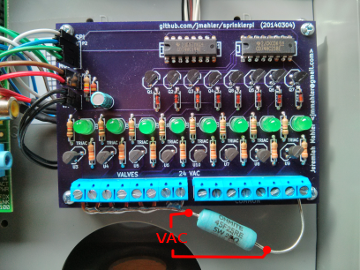
\includegraphics[scale=0.8]{img/contdrv-inst-03-load.png}
\end{center}
\caption{Control driver with test bridge installed.
The AC voltage drop is measured by testing at either side
of the load.}
\label{fig:contdrv-load}
\end{figure}

\begin{figure}[hbp!]
\begin{center}
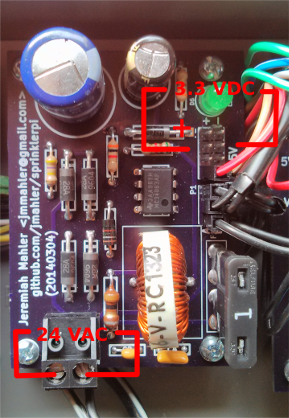
\includegraphics[scale=0.5,angle=0]{img/power-inst-03.png}
\end{center}
\caption{Power supply test points. In the upper right is 3.3 volts DC.
In the lower left is 24 volts AC.}
\label{fig:ps-test}
\end{figure}

\item Test Results \\
	\vspace{1em}
	With three valves on, one in each group, the voltage drop
	across each test bridge load should be: $9.5\pm0.5$ volts AC. \\
	\vspace{1em}
	\begin{tabular}{|c|c|c|c|c|}
		\hline
		Group & Valve	& Voltage Drop		& Pass/Fail & Notes \\
		\hline
		1 & 1 & & P \quad F & \hspace{20em} \\
		\hline
		2 & 1 && P \quad F & \\
		\hline
		3 & 1 && P \quad F & \\
		\hline
	\end{tabular}

	\vspace{1em}
	With the three valves on, the power supply should provide
	$24\pm4.8$ volts AC and $3.3\pm0.3$ volts DC (Figure \ref{fig:ps-test}). \\
	\vspace{1em}
	\begin{tabular}{|c|c|c|c|}
		\hline
		Test  & Value & Pass/Fail & Notes \\
		\hline
		3.3 volts DC & \hspace{5em} & P \quad F & \hspace{20em} \\
		\hline
		24 volts AC & & P \quad F & \\
		\hline
	\end{tabular}

\end{enumerate}
% }}}

% {{{ Valve Load Test
\clearpage
\subsection{Valve Load Test}

\begin{enumerate}
\item Equipment Required
	\begin{itemize}
	\item 110 volts AC power outlet (NEMA 5-15R).
	\item PC with Internet access and a web browser.
	\item Three Control/Driver test bridges (25 $\Omega$, 5 Watt).
	\item Digital multi meter.
	\end{itemize}
\item Input
	\begin{itemize}
	\item User actuation of valves using manual mode of web interface.
	\end{itemize}
\item Output
	\begin{itemize}
	\item $9.5\pm0.5$ volts AC across test bridge resistor when on.
	\end{itemize}

\item Test Description \\
\vspace{0.5em}

In this test the valve output for a control/driver is connected
to a test bridge (Figure \ref{fig:contdrv-load}) which places
it under a load.
Then each valve is manually operated from the web interface and
voltage drop across the load is measured to verify that the
correct amount of current is being drawn.

One valve should be on in each group during the entire test
to ensure the worst case load.
The voltage drop across the test bridge load should be: $9.5\pm0.5$ volts AC. \\

\item Test Results \\
	\vspace{1em}

	\begin{tabular}{|c|c|c|c|c|}
		\hline
		Group & Valve & Voltage Drop & Pass/Fail & Notes \\
		\hline
		1 & 1 &  & P \quad F & \hspace{20em} \\
		\hline
		1 & 2 &  & P \quad F & \\
		\hline
		1 & 3 &  & P \quad F & \\
		\hline
		1 & 4 &  & P \quad F & \\
		\hline
		1 & 5 &  & P \quad F & \\
		\hline
		1 & 6 &  & P \quad F & \\
		\hline
		1 & 7 &  & P \quad F & \\
		\hline
		1 & 8 &  & P \quad F & \\
		\hline
		\hline
		2 & 1 &  & P \quad F & \\
		\hline
		2 & 2 &  & P \quad F & \\
		\hline
		2 & 3 &  & P \quad F & \\
		\hline
		2 & 4 &  & P \quad F & \\
		\hline
		2 & 5 &  & P \quad F & \\
		\hline
		2 & 6 &  & P \quad F & \\
		\hline
		2 & 7 &  & P \quad F & \\
		\hline
		2 & 8 &  & P \quad F & \\
		\hline
		\hline
		3 & 1 &  & P \quad F & \\
		\hline
		3 & 2 &  & P \quad F & \\
		\hline
		3 & 3 &  & P \quad F & \\
		\hline
		3 & 4 &  & P \quad F & \\
		\hline
		3 & 5 &  & P \quad F & \\
		\hline
		3 & 6 &  & P \quad F & \\
		\hline
		3 & 7 &  & P \quad F & \\
		\hline
		3 & 8 &  & P \quad F & \\
		\hline
	\end{tabular}

\end{enumerate}
% }}}

% {{{ Scheduler Queuing Test
\clearpage
\subsection{Scheduler Queuing Test}

\begin{enumerate}
\item Equipment Required
	\begin{itemize}
	\item 110 volts AC power outlet (NEMA 5-15R).
	\item Computer with web browser and network connection.
	\end{itemize}
\item Input
	\begin{itemize}
	\item Schedule time and duration to run valve.
	\end{itemize}
\item Output
	\begin{itemize}
	\item Valve starts at expected time $\pm5$ seconds.
	\item Valves run for correct duration of time $\pm1$ second.
	\item Only one valve per group on at a time.
	\end{itemize}

\item Test Description \\
\vspace{0.5em}

This tests the scheduler queuing mechanism by starting multiple
operations in one group simultaneously.
Each operation should be completed and run for the expected amount
of time. Note, the order of operations is not guaranteed.

The LED valve indicators can be used to determine when the valve is on.

For a single group, configure it to start three different valves
at the same start time as shown in Figure \ref{fig:www-schedule_test1}.
The start time should be adjusted to some future time.
The run time can be any small amount such as 30 seconds. \\

\begin{framed}
\textbf{CAUTION}: The start time is relative to the time zone where
the server is installed and is not necessarily the same as the
time zone where it is being accessed from.
\end{framed}

\begin{figure}[hbp!]
\begin{center}
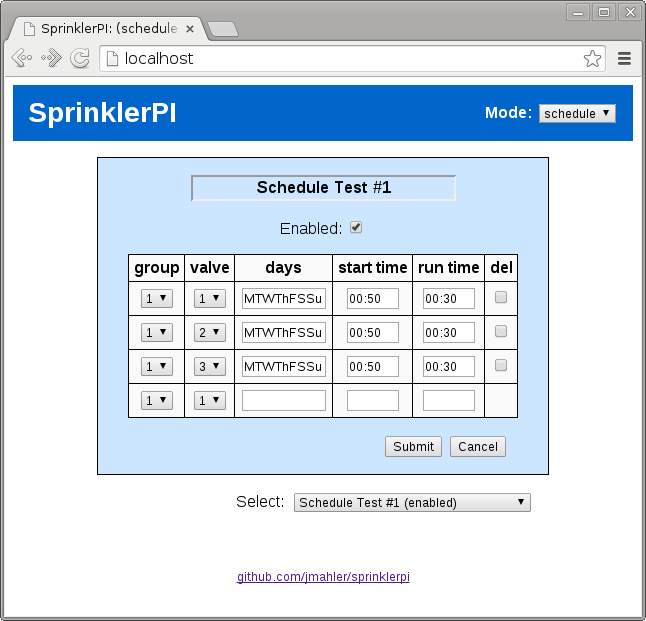
\includegraphics[scale=0.5]{img/www-schedule_test1}
\end{center}
\caption{Schedule configured to start three valves in one group
	simultaneously.}
\label{fig:www-schedule_test1}
\end{figure}

\item Test Results \\
	\vspace{1em}

	\vspace{1em}
	\begin{center}
	\begin{tabular}{|c|c|c|c|c|c|c|}
		\hline
		Group & Valve & Start Time & Run Time & Stop Time & Duration & Pass/Fail \\
		\hline
		1 & 1 & 		& 00:30 & & & P \quad F \\
		\hline
		1 & 2 & (same) & 00:30 & & & P \quad F \\
		\hline
		1 & 3 & (same) & 00:30 & & & P \quad F \\
		\hline
		\hline
		\multicolumn{7}{|c|}{Notes} \\
		\multicolumn{7}{|c|}{} \\
		\multicolumn{7}{|c|}{} \\
		\multicolumn{7}{|c|}{} \\
		\multicolumn{7}{|c|}{} \\
		\hline
	\end{tabular}
	\end{center}

\end{enumerate}

% }}}

% {{{ Scheduler Concurrency Test
\clearpage
\subsection{Scheduler Concurrency Test}

\begin{enumerate}
\item Equipment Required
	\begin{itemize}
	\item 110 volts AC power outlet (NEMA 5-15R).
	\item Computer with web browser and network connection.
	\end{itemize}
\item Input
	\begin{itemize}
	\item Schedule time and duration to run valve.
	\end{itemize}
\item Output
	\begin{itemize}
	\item Valve starts at expected time $\pm5$ seconds.
	\item Valves run for correct duration of time $\pm1$ second.
	\item Valves in different groups run concurrently.
	\end{itemize}

\item Test Description \\
\vspace{0.5em}

This tests the scheduler queuing mechanism by starting
operations in different groups simultaneously.
Each operation should be completed and run for the expected length of time.
Valves in different groups should run concurrently.

The LED valve indicators can be used to determine when the valve is on.

For each group, configure it to start a valve 
at the same time as shown in Figure \ref{fig:www-schedule_test2}.
The start time should be adjusted to some future time relative
to a particular local time.
The run time can be any small amount such as 30 seconds. \\

\begin{framed}
\textbf{CAUTION}: The start time is relative to the time zone where
the server is installed and is not necessarily the same as the
time zone where it is being accessed from.
\end{framed}

\item Test Results \\
	\vspace{1em}
	\begin{figure}[hbp!]
	\begin{center}
	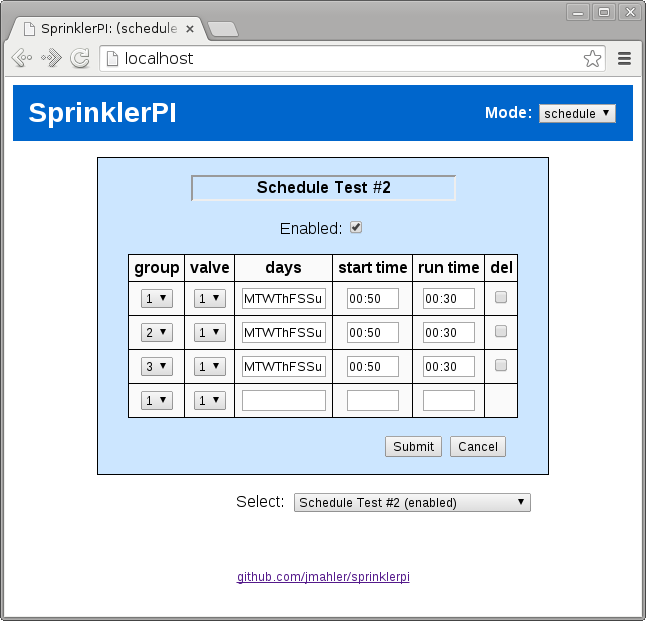
\includegraphics[scale=0.5]{img/www-schedule_test2}
	\end{center}
	\caption{Schedule configured to start three valves in different groups
		simultaneously.}
	\label{fig:www-schedule_test2}
	\end{figure}

	\vspace{1em}
	\begin{center}
	\begin{tabular}{|c|c|c|c|c|c|c|}
		\hline
		Group & Valve & Start Time & Run Time & Stop Time & Duration & Pass/Fail \\
		\hline
		1 & 1 & & 00:30 & & & P \quad F \\
		\hline
		2 & 1 & (same) & 00:30 & & & P \quad F \\
		\hline
		3 & 1 & (same) & 00:30 & & & P \quad F \\
		\hline
		\hline
		\multicolumn{7}{|c|}{Notes} \\
		\multicolumn{7}{|c|}{} \\
		\multicolumn{7}{|c|}{} \\
		\multicolumn{7}{|c|}{} \\
		\multicolumn{7}{|c|}{} \\
		\hline
	\end{tabular}
	\end{center}

\end{enumerate}

% }}}

% }}}

%\clearpage
%\appendix

% References
\clearpage
\printbibliography[heading=bibintoc]

\end{document}

